\section{Discrete Mathematics}
\begin{questions}
	\subsection{Definitions}
	\question Define: 
	\begin{parts}
		\part derangement
		\part digraph
		\part walk 
		\part trail
		\part tree
		\part hamiltonian cycle
		\part bipartite graph
		\part heuristic algorithm 
	\end{parts}
	\subsection{Classification of problems}
	\question You need to be at school by $0837$ but don't want to leave your house before $0730$. Within the context of this example, can you explain the following terms: 
	\begin{parts}
		\part existence
		\part construction
		\part enumeration
		\part optimisation 
	\end{parts} 
	\subsection{Sets and Counting}
	\question Three sets, A, B and C have 28, 28 and 22 members, $n(A\cup B \cup C) = 42$, $n(A \cap B) = 17$, $n(A \cap C) = 13$ and $n(B \cap C) = 15$. 
	\begin{parts}
		\part What is $n(A\cap B \cap C)$?
		\part If $n(\varepsilon) = 50$, what is $n(B')$?
	\end{parts}
	\question Prove that if you pick three integers at random, a pair of them will add up to an even number. \begin{solution}pigeonhole\end{solution}
	\question In a race involving 8 athletes, how many different ways can the medals for first, second and third be awarded? 
	\question In a class of 12 students, how many ways can they be split into 
	\begin{parts}
		\part 4 teams of 3;  
		\part 3 teams of 4?
	\end{parts}  

	\question How many derangements are there of the word ``NOTE''? 
	\begin{solution}
	\begin{align}
	!n &= (n-1)(!(n-1)+!(n-2)) \\
	!4 &= 9
	\end{align}
	\end{solution}
	\subsection{Graphs}
	\question A graph has nodes with degree ${2, 2, 3, 3, 4, 4}$:
	\begin{parts}
		\part Draw a possible layout for this graph, the nodes should be labelled A--F.
		\part Identify a semi-Eulerian route through your graph. 
		\part Explain whether or not your graph is simple. 		
	\end{parts}
	\question Show that there are exactly six non-isomorphic trees on six vertices. \begin{solution}Brute force \textit{https://math.stackexchange.com/questions/413792/trees-on-six-vertices}\end{solution}

	\question Using this graph: 

	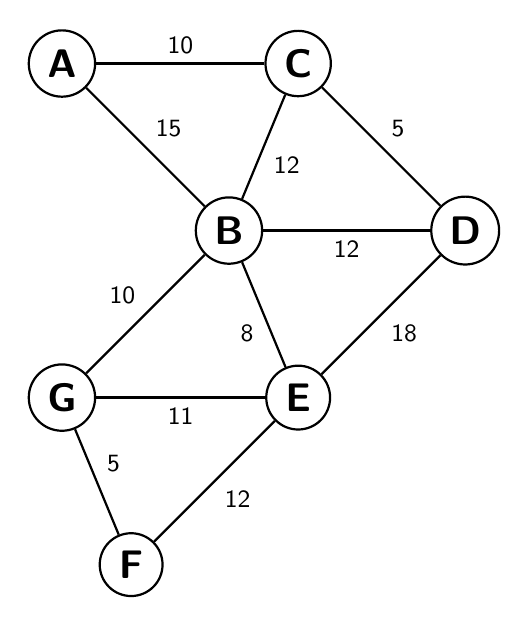
\begin{tikzpicture}[auto, node distance=3cm, every loop/.style={},
                    thick,main node/.style={circle,draw,font=\sffamily\Large\bfseries}]

		  \node[main node] (A) {A};
		  \node[main node] (B) [below right of=A] {B};
		  \node[main node] (C) [right of=A] {C};
		  \node[main node] (D) [right of=B] {D};
		  \node[main node] (E) [below left of=D] {E};
		  \node[main node] (G) [below left of=B] {G};
		  \node[main node] (F) [below left of=E] {F};

		  \path[every node/.style={font=\sffamily\small}]
		    (A) edge node  {10} (C)
		        edge node {15} (B)
		    (C) edge node {12} (B)
		        edge node {5} (D)
		    (D) edge node {12} (B)
		        edge node {18} (E)
		    (E) edge node {8} (B)
		        edge node {11} (G)
		        edge node {12} (F)
		    (G) edge node {10} (B)
		        edge node {5} (F)
		    ;
	\end{tikzpicture}

	\begin{parts}
		\part Apply Prim's algorithm and starting at `A', listing the order in which the nodes should be selected. What is the weight of your minimum spanning tree? 
		\part Apply Kruskal's algorithm, listing the order in which the nodes should be selected. What is the weight of your minimum spanning tree? 

	\end{parts}
\end{questions}